\chapter{Vorgehen}
Mit der in der Projektarbeit entwickelten Harvesterschaltung kann per Bluetooth Smart auf dem Android-Endgerät die Geschwindigkeit ausgegeben werden.

\section{Inbetriebnahme des Modells der Machbarkeitsstudie}



\subsubsection{Reduktion Kapazität Harvesting-Schaltung}
In der Machbarkeitsstudie ist nach dem Gleichrichter ein Kondensator von 470 uF nachgeschaltet. Dieser glättet die Spannungspulse zu Rippeln. Ives von EMMicroelectronics rät den Kondensator um den Faktor 10 zu verkleineren, da die nachfolgende Energiemanagementschaltung sonst nicht mit Sicherheit ordnungsgemäss funktioniert. 

Aus diesem Grund wird die Rippelspannung am Ausgangs der Harvesterschaltung mit kleineren Kondensatoren gemessen. Das Messprotokoll befindet sich im Anhang.

\subsubsection*{Messaufbau}

\begin{figure}
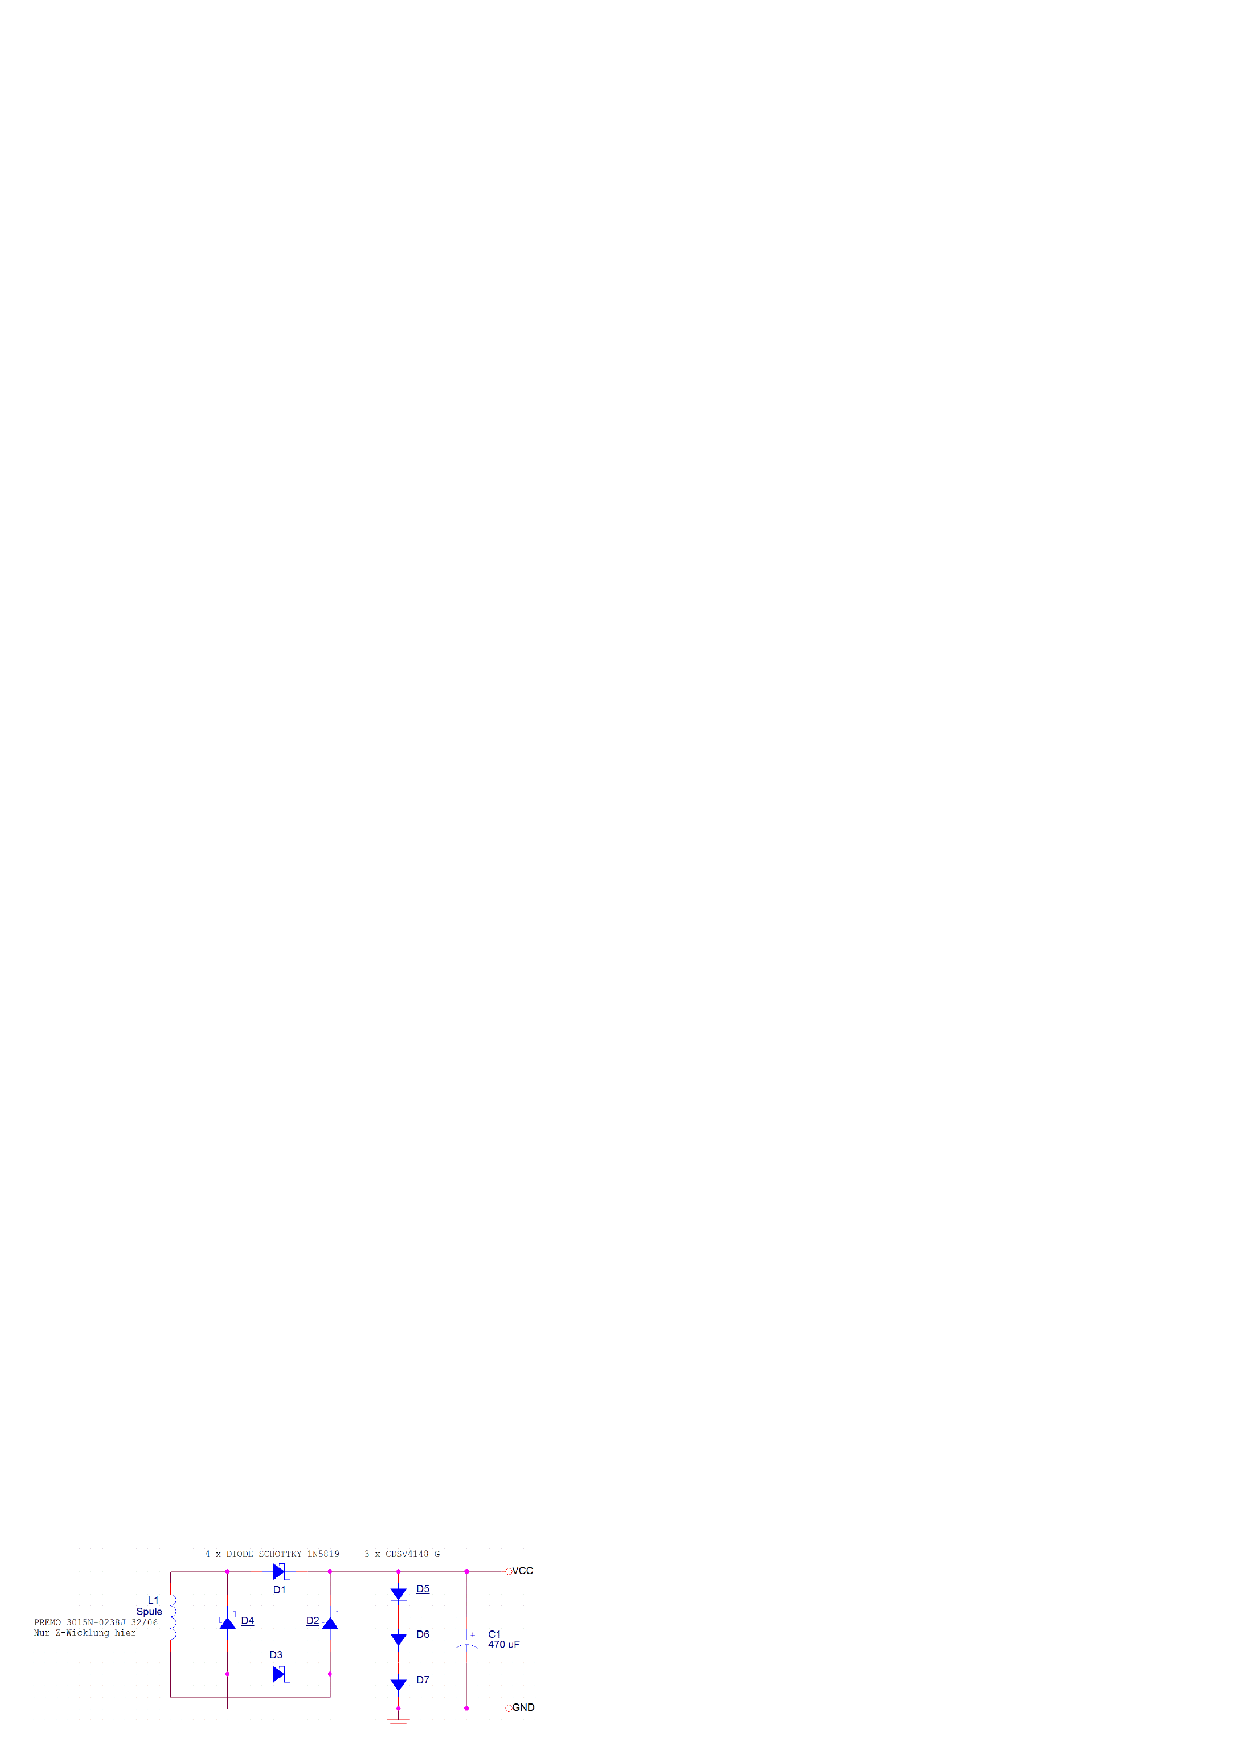
\includegraphics[bb = 0 0 100 100]{3Vorgehen/imag/messschaltungHarvesterschaltung.gif}
\caption{Messschaltung}
\end{figure}

\subsubsection*{Resultate}

\begin{figure}
\includegraphics[bb = 0 0 100 100]{3Vorgehen/imag/10uF.PNG}
\caption{Rippelspannung mit 10 uFKondensator}
\end{figure}

\begin{figure}
\includegraphics[bb = 0 0 100 100]{3Vorgehen/imag/47uF.PNG}
\caption{Rippelspannung mit 47 uFKondensator}
\end{figure}

\pagebreak 
\subsubsection{Messungen Energy Management Board}

 
Es zeigt sich, dass der LTS nicht geladen wird . Und es zeigt sich, dass das EM-Board nicht zu regulieren beginnt.


Lastverhalten wie Sensortag






\pagebreak
\subsubsection{Messungen Sensortag}
Ziel: Energieverbrauch kennen.

Unterschied zwischen dem Programmierten Sensortag des Prototypen und dem neuen Sensortag.




\section{Layout Print}

\section{Kommunikation Bluetooth Low Energy}

\section{Energieoptimierung}



\section{Applikationsentwicklung}

\section{Option 1}






